\documentclass{beamer}
\usepackage[utf8]{inputenc}

\usepackage{amsmath}
\usepackage{graphicx}
\usepackage{url}
\usepackage{fancyvrb}
\usepackage{xcolor}
\usepackage{adjustbox}

\usetheme{Madrid}
\usecolortheme{seahorse}

\usepackage{inconsolata}
\usepackage[scaled]{helvet}
\renewcommand*\familydefault{\sfdefault}
\usepackage[T1]{fontenc}

\usepackage{listings}
\usepackage{color}

\definecolor{codegreen}{rgb}{0,0.6,0}
\definecolor{codegray}{rgb}{0.5,0.5,0.5}
\definecolor{codepurple}{rgb}{0.58,0,0.82}
\definecolor{backcolour}{rgb}{0.95,0.95,0.92}

\mode<presentation>

\definecolor{orange}{HTML}{BC2E07}

\usepackage{hyperref}
\hypersetup{
    colorlinks,
    linkcolor=orange,
    urlcolor=blue
}

\lstdefinestyle{mystyle}{
    language=C++,
    basicstyle=\ttfamily\footnotesize,
    backgroundcolor=\color{backcolour},
    commentstyle=\color{codegreen},
    keywordstyle=\color{magenta},
    numberstyle=\tiny\color{codegray},
    stringstyle=\color{codepurple},
    breakatwhitespace=false,
    breaklines=true,
    captionpos=b,
    keepspaces=true,
    numbers=left,
    numbersep=5pt,
    showspaces=false,
    showstringspaces=false,
    showtabs=false,
    tabsize=2
}

\usepackage{datetime}
\newdate{date}{23}{11}{2015}

\title{Lab \# 14: Functions - IV}
\subtitle{EC-102 -- Computer Systems and Programming}

\author{Usman Ayub Sheikh}
\institute{School of Mechanical and Manufacturing Engineering (SMME), \\ National University of Sciences and Technology (NUST)}
\date{\displaydate{date}}

\begin{document}

\begin{frame}
    \titlepage
\end{frame}

\begin{frame}
    \frametitle{Outline}
        \tableofcontents
\end{frame}

\begin{frame}\frametitle{Overloaded Functions}
    \section{Overloaded Functions} % (fold)
    \label{sec:overloaded_functions}
    \subsection{Definition} % (fold)
    \label{sub:definition}
    \begin{columns}
        \column{0.55\textwidth}
        A function that
        \begin{itemize}
            \item Appears to perform different activities depending on the kind of data sent to it
            \item Performs one operation on one kind of data but another operation on a different kind
        \end{itemize}
        \column{0.45\textwidth}
        \begin{figure}
            \centering
            
\includegraphics[scale=0.25]{how}
        \end{figure}
    \end{columns}
\end{frame}

\begin{frame}[fragile]\frametitle{Different Number of Arguments}
    \subsection{Different Number of Arguments} % (fold)
    \label{sub:different_number_of_arguments}
    \lstset{style=mystyle}
\begin{lstlisting}
// demonstrates function overloading
#include <iostream>
using namespace std;

void repchar();
void repchar(char);
void repchar(char, int);

int main()
{
    repchar();
    repchar('-');
    repchar('~', 10);
}
\end{lstlisting}
\end{frame}

\begin{frame}[fragile]\frametitle{Different Number of Arguments}
    \lstset{style=mystyle}
\begin{lstlisting} [firstnumber=15]
// displays 45 asterisks
void repchar()
{
    for(int i = 0; i < 45; i++)
    {
        cout << '*';
    }
    cout << endl;
}

// displays 45 copies of a specified character
void repchar(char ch)
{
    for(int i = 0; i < 45; i++)
    {
        cout << ch;
    }
    cout << endl;
}
\end{lstlisting}
\end{frame}

\begin{frame}[fragile]\frametitle{Different Number of Arguments}
    \lstset{style=mystyle}
\begin{lstlisting} [firstnumber=34]
// displays specified number of copies of a specified character
void repchar(char ch, int n)
{
    for(int i = 0; i < n; i++)
    {
        cout << ch;
    }
    cout << endl;
}
\end{lstlisting}
\end{frame}

\begin{frame}[fragile]\frametitle{Different Kinds of Arguments}
    \subsection{Different Kinds of Arguments} % (fold)
    \label{sub:different_kinds_of_arguments}
    \lstset{style=mystyle}
\begin{lstlisting}
// demonstrates overloaded functions
#include <iostream>
using namespace std;

struct Distance
{
    int feet;
    float inches;
};

void engldisp(Distance);
void engldisp(float);
\end{lstlisting}
\end{frame}

\begin{frame}[fragile]\frametitle{Different Kinds of Arguments}
    \lstset{style=mystyle}
\begin{lstlisting} [firstnumber=14]
int main()
{
    Distance d1;
    float d2;

    cout << "Enter feet: "; cin >> d1.feet;
    cout << "Enter inches: "; cin >> d1.inches;

    cout << "Enter entire distance in inches: "; cin >> d2;

    cout << "\nd1 = ";
    engldisp(d1);
    cout << "\nd2 = ";
    engldisp(d2);
    cout << endl;
    return 0;
}
\end{lstlisting}
\end{frame}

\begin{frame}[fragile]\frametitle{Different Kinds of Arguments}
    \lstset{style=mystyle}
\begin{lstlisting} [firstnumber=31]
// displays structure of type Distance in feet and inches
void engldisp(Distance dd)
{
    cout << dd.feet << "\'-" << dd.inches << "\"";
}

// display variable of type float in feet and inches
void engldisp(float dd)
{
    int feet = dd / 12;
    float inches = dd - feet * 12;
    cout << feet << "\'-" << inches << "\"";
}
\end{lstlisting}
\end{frame}

\begin{frame}\frametitle{Recursion}
    \section{Recursion} % (fold)
    \label{sec:recursion}
    \subsection{What is it?} % (fold)
    \label{sub:what_is_it_}
    \begin{columns}
        \column{0.55\textwidth}
        \begin{itemize}
            \item A function calling itself
            \item When used correctly, this technique can be surprisingly powerful
        \end{itemize}
        \column{0.45\textwidth}
        \begin{figure}
            \centering
            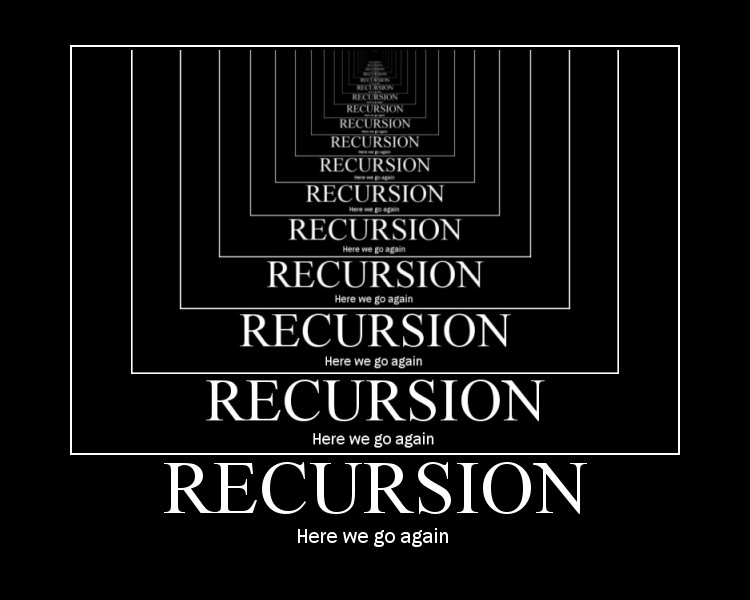
\includegraphics[scale=0.2]{recursion}
        \end{figure}
    \end{columns}
\end{frame}

\begin{frame}[fragile]\frametitle{How to Use Recursion?}
    \subsection{How to Use it?} % (fold)
    \label{sub:how_to_use_it_}
    \lstset{style=mystyle}
\begin{lstlisting}
// calculates factorials using recursion
#include <iostream>
using namespace std;

unsigned long factfunc(unsigned long);

int main()
{
    int n;
    unsigned long fact;

    cout << "Enter an integer: "; cin >> n;
    fact = factfunc(n);
    cout << "Factorial of " << n << " is: " << fact << endl;
    return 0;
}
\end{lstlisting}
\end{frame}

\begin{frame}[fragile]\frametitle{How to Use Recursion?}
    \lstset{style=mystyle}
\begin{lstlisting} [firstnumber=19]
unsigned long factfunc(unsigned long n)
{
    if(n > 1)
    {
        return n * factfunc(n - 1);
    }
    else
    {
        return 1;
    }
}
\end{lstlisting}
\end{frame}

\begin{frame}\frametitle{How to Use Recursion?}
    \begin{columns}
        \column{0.55\textwidth}
        \begin{itemize}
            \item Every recursive function must be provided with a way to end the recursion
            \item Otherwise it will call itself forever and crash the program
        \end{itemize}
        \column{0.45\textwidth}
        \begin{figure}
            \centering
            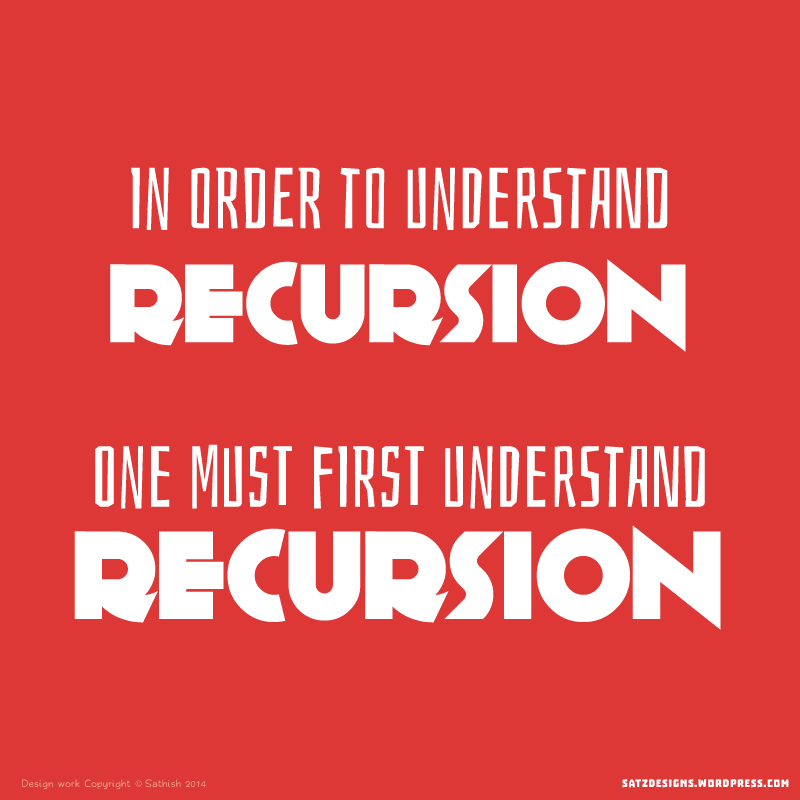
\includegraphics[scale=0.18]{recurse.jpg}
        \end{figure}
    \end{columns}
\end{frame}

\begin{frame}\frametitle{Default Arguments}
    \section{Default Arguments} % (fold)
    \label{sec:default_arguments}
    \subsection{What?} % (fold)
    \label{sub:what_}
    \begin{itemize}
        \item A function can also be called without specifying all of its arguments
        \item But this won't work on just any function
        \item The function declaration must provide default values for those arguments that are not specified
    \end{itemize}
\end{frame}

\begin{frame}[fragile]\frametitle{How to Use Default Arguments?}
    \subsection{How?} % (fold)
    \label{sub:how_}
    \lstset{style=mystyle}
\begin{lstlisting}
// demonstrates missing and default arguments
#include <iostream>
using namespace std;

void repchar(char = '*', int = 45);

int main()
{
    repchar();
    repchar('+');
    repchar('^', 30);
    return 0;
}
\end{lstlisting}
\end{frame}

\begin{frame}[fragile]\frametitle{How to Use Default Arguments?}
    \lstset{style=mystyle}
\begin{lstlisting} [firstnumber=14]
void repchar(char ch, int n)
{
    for(int j = 0; j < n; j++)
    {
        cout << ch;
    }
    cout << endl;
}
\end{lstlisting}
\end{frame}

\begin{frame}\frametitle{Why Use Default Arguments?}
\subsection{Why?} % (fold)
\label{sub:why_}
\begin{itemize}
    \item They are useful if you don't want to to go through the trouble of writing arguments that have the same value most of the time
    \item They are also useful if the programmer decides to increase the capability of a function by adding another argument
\end{itemize}
\end{frame}

\begin{frame}\frametitle{Exercise 1}
\section{Exercises} % (fold)
\label{sec:exercises}
\subsection{Exercise 1} % (fold)
\label{sub:exercise_1}
Create a series of \textbf{overloaded functions} named as \texttt{firstn} such that
\begin{itemize}
    \item if \texttt{firstn} is called without any argument, first 10 numbers divisible by 2 are printed,
    \item if \texttt{firstn} is called with one argument, first 10 numbers divisible by the specified number are printed, and
    \item if \texttt{firstn} is called with two arguments, first m numbers divisible by n are printed.
\end{itemize}
\end{frame}

\begin{frame}\frametitle{Exercise 2}
\subsection{Exercise 2} % (fold)
\label{sub:exercise_2}
Create a function named as \texttt{firstn} using \textbf{default arguments} such that
\begin{itemize}
    \item if \texttt{firstn} is called without any argument, first 10 numbers divisible by 2 are printed,
    \item if \texttt{firstn} is called with one argument, first 10 numbers divisible by the specified number are printed, and
    \item if \texttt{firstn} is called with two arguments, first m numbers divisible by n are printed.
\end{itemize}
\end{frame}

\begin{frame}\frametitle{Exercise 3}
\subsection{Exercise 3} % (fold)
\label{sub:exercise_3}
Create a function named as \texttt{backward\_counting} using \textbf{recursion} that
\begin{itemize}
    \item Takes an integer as an argument, and
    \item Prints out backward counting starting at the specified number
\end{itemize}
\end{frame}

\begin{frame}\frametitle{Exercise 4}
\subsection{Exercise 4} % (fold)
\label{sub:exercise_4}
\textbf{Part 1:} \\
Create a function named as \texttt{fibonacci} using \textbf{recursion} that
\begin{itemize}
    \item Takes a number \texttt{n} as an argument, and
    \item returns $n^{th}$ Fibonacci number
\end{itemize}

\vspace{0.3cm}

Fibonacci sequence goes as follows: \texttt{1, 1, 2, 3, 5, 8, 13, ...} \\

\vspace{0.3cm}

The function should work as follows: \\
\texttt{fibonacci(0)} and {fibonacci(1)} should equal 1, \\
\texttt{fibonacci(5)} should equal 8, and so on. \\

\vspace{0.3cm}

\textbf{Part 2:} \\
Write a program that
\begin{itemize}
    \item exercises this functions by obtaining a number \texttt{x} from the user, and
    \item printing out first \texttt{x} numbers in the Fibonacci sequence
\end{itemize}

\end{frame}

\end{document}